\section{Auswertung}
\label{sec:Auswertung}

\subsection{Kompensation des Erdmagnetfeldes}
Die vertikale Komponente des Erdmagnetfeldes wird durch die vertikale Spule kompensiert.
Das Magnetfeld eines Helmholtzspulenpaar berechnet sich mit dem Spulenstrom $I$, der Windungszahl pro Spule $N$ und dem Spulenradius $R$.

\begin{equation}
  B = \mu_0\frac{8\cdot IN}{\sqrt{125}\cdot R}
  \label{eq:bfeld}
\end{equation}

Für die Vertikalspule gilt $N=20$ und $R=11.735\,$cm.
Bei dem Spulenstrom von $I=200\,$mA ist der Einfluss des Erdmagnetfeldes am geringsten.
Daraus ergibt sich die vertikale Komponente des Erdmagnetfeldes zu $B_{vert}=30.65\,\mu$m.

\subsection{Landé-Faktoren und Kernspins}
Die aufgenommenen RF-Frequenzen und Ströme für Horizontal und Sweepspule, bei denen die Transparenz ein Minimum hat, sind in Tabelle \ref{tab:rf} zu finden.
\begin{table}
  \centering
  \caption{RF-Frequenzen und Ströme der Horizonatal- und Sweepspule.}
  \label{tab:rf}
  \begin{tabular}{c | c | c | c | c}
    \toprule
    $\nu_{RF}$/kHz & $I_{H,87}$/A & $I_{S,87}$/A& $I_{H,85}$/A& $I_{S,85}$/A \\
    \midrule
    100.0 & 0.0 & 0.391 & 0.0 & 0.512 \\
    200.0 & 0.0 & 0.628 & 0.0 & 0.865 \\
    300.0 & 0.009 & 0.445 & 0.009 & 0.8 \\
    400.0 & 0.033 & 0.4 & 0.033 & 0.872 \\
    500.0 & 0.063 & 0.22 & 0.063 & 0.81 \\
    600.0 & 0.0915 & 0.078 & 0.0915 & 0.789 \\
    700.0 & 0.099 & 0.09 & 0.0989 & 0.917 \\
    800.0 & 0.118 & 0.183 & 0.159 & 0.375 \\
    900.0 & 0.126 & 0.23 & 0.1881 & 0.36 \\
    1000.0 & 0.149 & 0.209 & 0.219 & 0.245 \\
    \bottomrule
  \end{tabular}
\end{table}
\FloatBarrier
Aus den oben stehenden Strömen wird mit Gleichung \ref{eq:bfeld} das Magnetfeld berechnet.
Für die Horizontalspule gilt $N=154$ und $R=15.79\,$cm, für die Sweepspule gilt $N=11$ und $R=16.39\,$cm.
Eine lineare Regression des Magnetfeldes gegen die eingestellte Frequenz liefert
\begin{align*}
  B_{87} &= (0.134\pm0.006)\,\mu\text{T/kHz}\cdot\nu + (4\pm3)\,\mu\text{T}\\
  B_{85} &= (0.198\pm0.006)\,\mu\text{T/kHz}\cdot\nu + (6.4\pm3.4)\,\mu\text{T}
\end{align*}
Die Daten mit den zugehörigen oben genannten Geraden sind in Abbildung \ref{fig:rf}
\begin{figure}
  \centering
  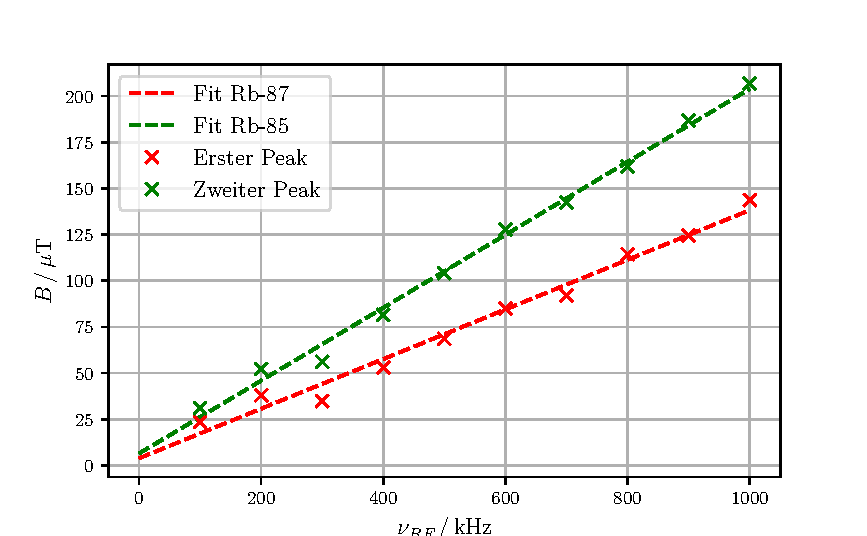
\includegraphics{plot1.pdf}
  \caption{Horizontales Magnetfeld gegen die Frequenz.}
  \label{fig:rf}
\end{figure}
\FloatBarrier
Gemäß Gleichung \ref{eq:??}%Gleichung der Übergangsenergie
folgen daraus die Landé-Faktoren.
\begin{align*}
  g_{\text{F,87}} &= 0.531\pm0.026\\
  g_{\text{F,87}} &= 0.362\pm0.010
\end{align*}
Jetzt wird mit Gleichung \ref{eq:??} %Gleichung für gj
$g_\text{J}$ berechnet.
Mit $S=\frac{1}{2}$, $L=0$ und $J=\frac{1}{2}$ folgt $g_\text{J} = 2.0023$.
Für die Kernspins gilt
\begin{equation}
  I = \frac{g_\text{J}}{2g_\text{F}-\frac{1}{2}}
\end{equation}
Damit folgen
\begin{align*}
  I_{87} &= 1.38\pm0.09 \\
  I_{85} &= 2.27\pm0.08
\end{align*}

\subsection{Isotopenverhältnis}
Abbildung \ref{fig:signal} zeigt ein typisches Signalbild.
Das Amplitudenverhältnis der beiden beobachteten Transparenzminima entspricht dem Isotopenverhältnis der untersuchten Probe.
\begin{figure}
  \centering
  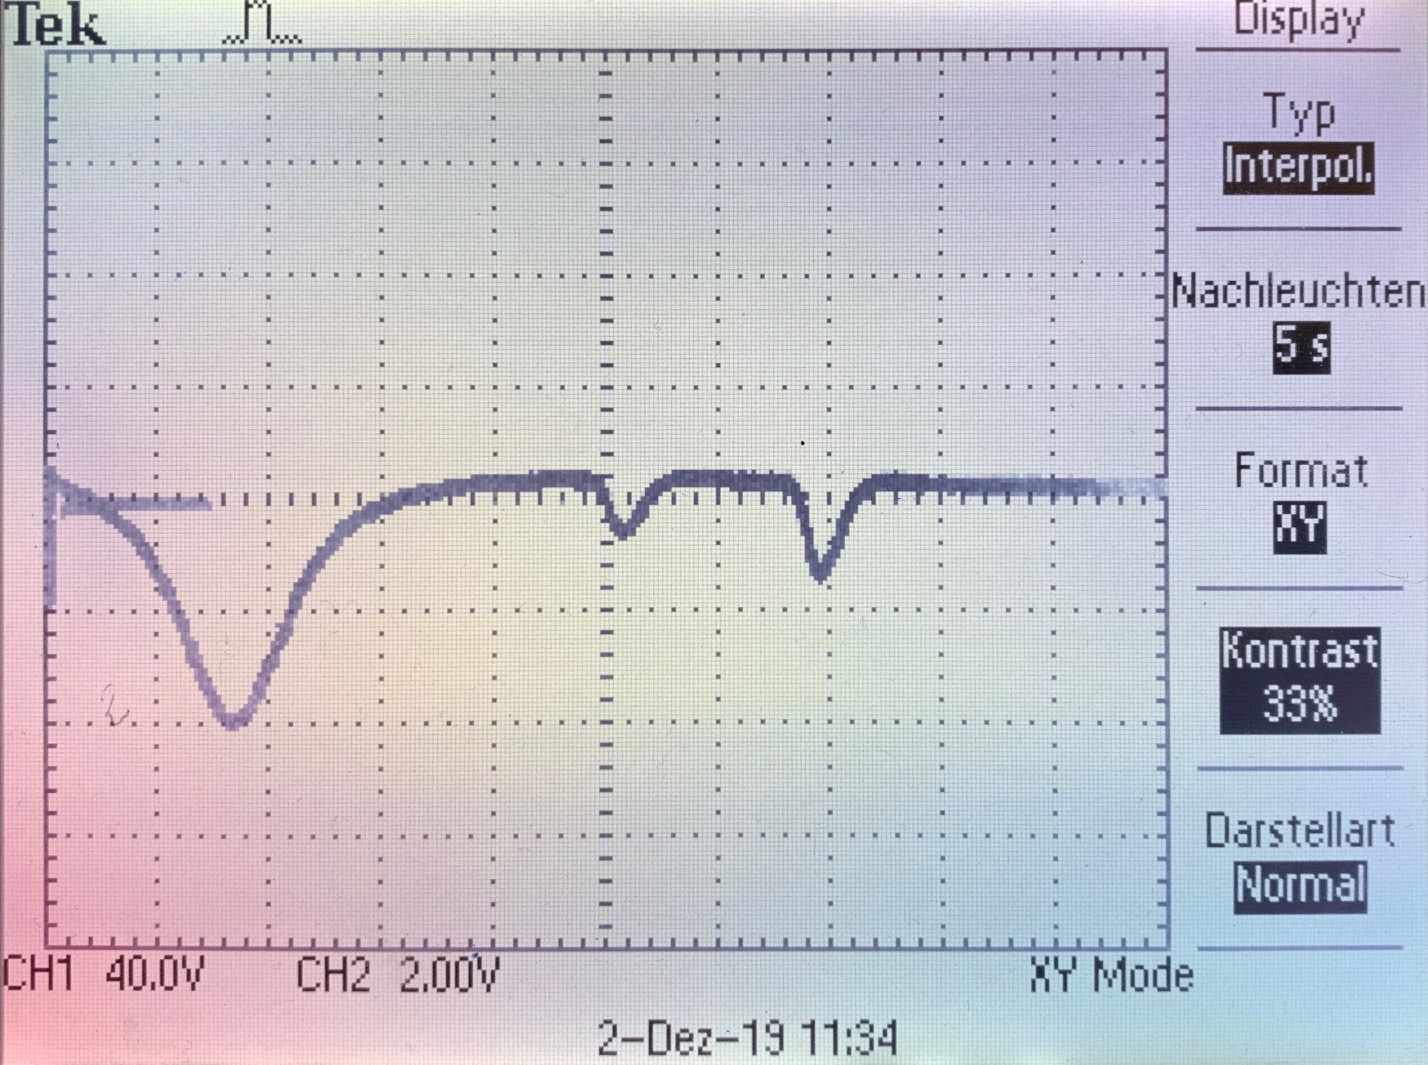
\includegraphics[width=\textwidth]{data/Signal.jpg}
  \caption{Oszilloskopbild bei $100\,$kHz.}
  \label{fig:signal}
\end{figure}
\FloatBarrier
\begin{align*}
  &\frac{N\left(^{85}\text{Rb}\right)}{N\left(^{87}\text{Rb}\right)}\\
  &=\frac{4.0\pm0.5}{2.0\pm0.5}\\
  &=2\pm0.75
\end{align*}
Die angenommene Abweichung kommt durch das nur bedingt genaue Ablesen der Amplituden.

\subsection{Quadratischer Zeeman-Effekt}
Im Folgenden wird der Einfluss des quadratischen Zeeman-Effekte untersucht. 
Dazu wird die Formel
\begin{equation}
  U_{\text{HF}}=g_{\text{F}}\mu_{\text{B}}B+g_{\text{F}}^2\mu_{\text{B}}^2B^2\frac{(1-2M_{\text{F}})}{\Delta E_{\text{Hy}}}-\ldots
  \label{eq:zeemanenergie}
\end{equation}
gegeben.
In linearer Näherung folgt für die Zeeman-Energie
\begin{align*}
  U_{\text{HF,87,linear}}&= (7.08\pm0.34)\cdot 10^{-28} J\\
  U_{\text{HF,85,linear}}&= (6.94\pm0.19)\cdot 10^{-28} J
\end{align*}
und in quadratischer Näherung
\begin{align*}
  U_{\text{HF,87,quad}}&= (2.49\pm0.24)\cdot 10^{-31} J\\
  U_{\text{HF,85,quad}}&= (1.06+/-0.06)\cdot 10^{-31} J
\end{align*}

\subsection{Untersuchung der transienten Effekte}
\begin{figure}
  \centering
  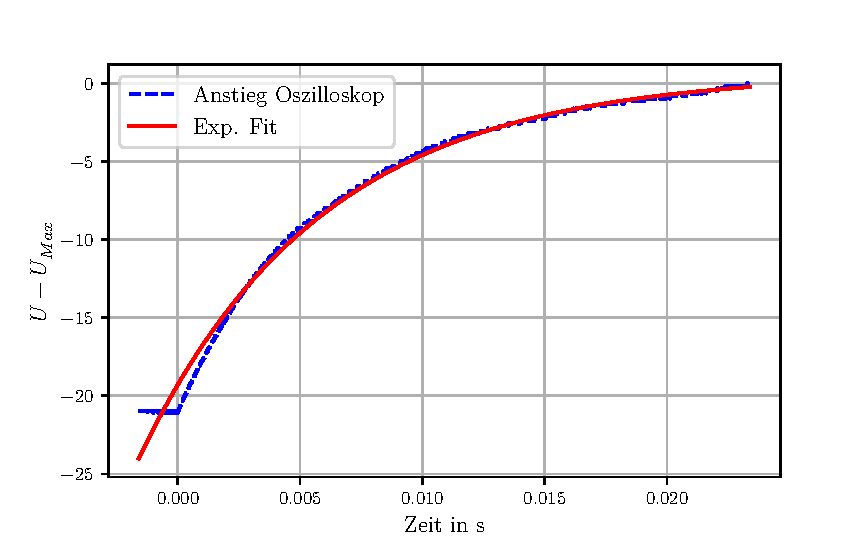
\includegraphics{anstieg.pdf}
  \caption{Oszilloskopdaten beim einschalten einer Rechteckspannung.}
  \label{fig:anstieg}
\end{figure}
\FloatBarrier
Abbildung \ref{fig:anstieg} zeigt den exponentiellen Anstieg der Transparenz
der Zelle auf der $^{85}$Rb-Resonanz beim Anlegen einer Rechteckspannung.
Die aufgenommenen Messwerte zur Untersuchung der Abhängigkeit von Schwingungsperiode 
und angelegter Hochfrequenzamplitude sind in Tabelle \ref{tab:periodendauer} aufgeführt. 
Die Anpassung von Hyperbelfunktionen der Form
\begin{equation}
  T=a+\frac{b}{U-c}
\end{equation}
%
an die Messwerte liefert
\begin{align*}
  T_{87}&=(-0.034\pm0.027)\,\text{ms}+\frac{(5.86\pm0.26)\,\text{msV}}{U-(-0.45\pm0.09)\,\text{V}} \\
  T_{85}&=(0.039\pm0.035)\,\text{ms}+\frac{(7.90\pm0.33)\,\text{msV}}{U-(-0.33\pm0.08)\,\text{V}}
\end{align*}
Daraus folgt das Verhältnis
\begin{align*}
  \frac{b_85}{b_87}=1.35\pm0.08
\end{align*}
\begin{table}
  \centering
  \caption{Gemessene Periodendauer bei eingestellter Hochfrequenzamplitude.}
  \label{tab:periodendauer}
  \begin{tabular}{c | c | c }
    \toprule
    $U$/V & $T_{87}$/ms & $T_{85}$/ms \\
    \midrule
    2.0 & 2.36 & 3.44 \\
    3.0 & 1.64 & 2.4 \\
    4.0 & 1.28 & 1.86 \\
    5.0 & 1.06 & 1.52 \\
    6.0 & 0.88 & 1.32 \\
    7.0 & 0.76 & 1.12 \\
    8.0 & 0.65 & 0.98 \\
    9.0 & 0.58 & 0.9 \\
    10.0 & 0.52 & 0.78 \\
    \bottomrule
  \end{tabular}
\end{table}
\FloatBarrier
\begin{figure}
  \centering
  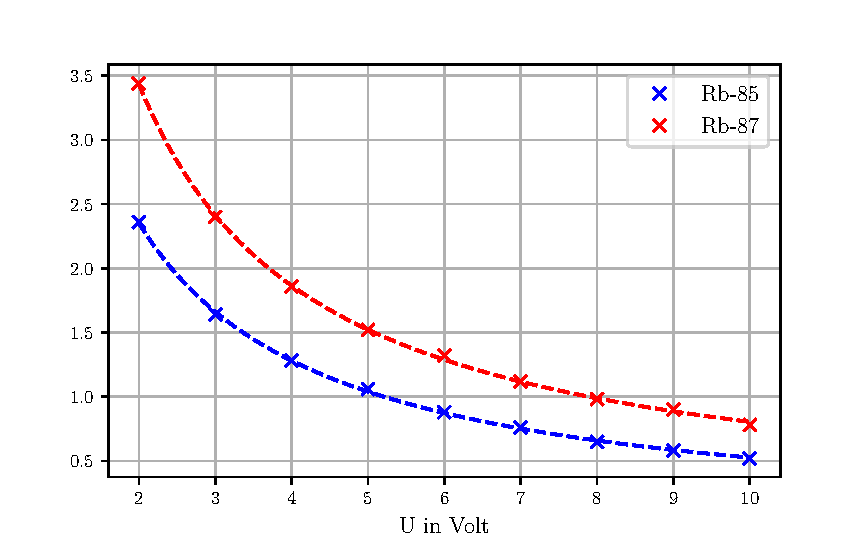
\includegraphics{perioden.pdf}
  \caption{Optimierte Hyperbelfunktionen and gemessene Daten gefittet.}
  \label{fig:perioden}
\end{figure}
\FloatBarrier